%% Experimental validation 
\frame{
\begin{tikzpicture}[remember picture,overlay]
\fill[blue1]
(current page.north west) rectangle ([xshift=0.51\textwidth,yshift=0.28\textheight]current page.west|-{pic cs:end});
\end{tikzpicture}

\begin{textblock}{0.5}(0.02,0.03)
	\textcolor{white}{
	\Large Experimental validation of X-DFA: Sedimenting particle suspension}
\end{textblock}

\begin{textblock}{0.6}(0.02,0.2)
\centering
\only<1>{
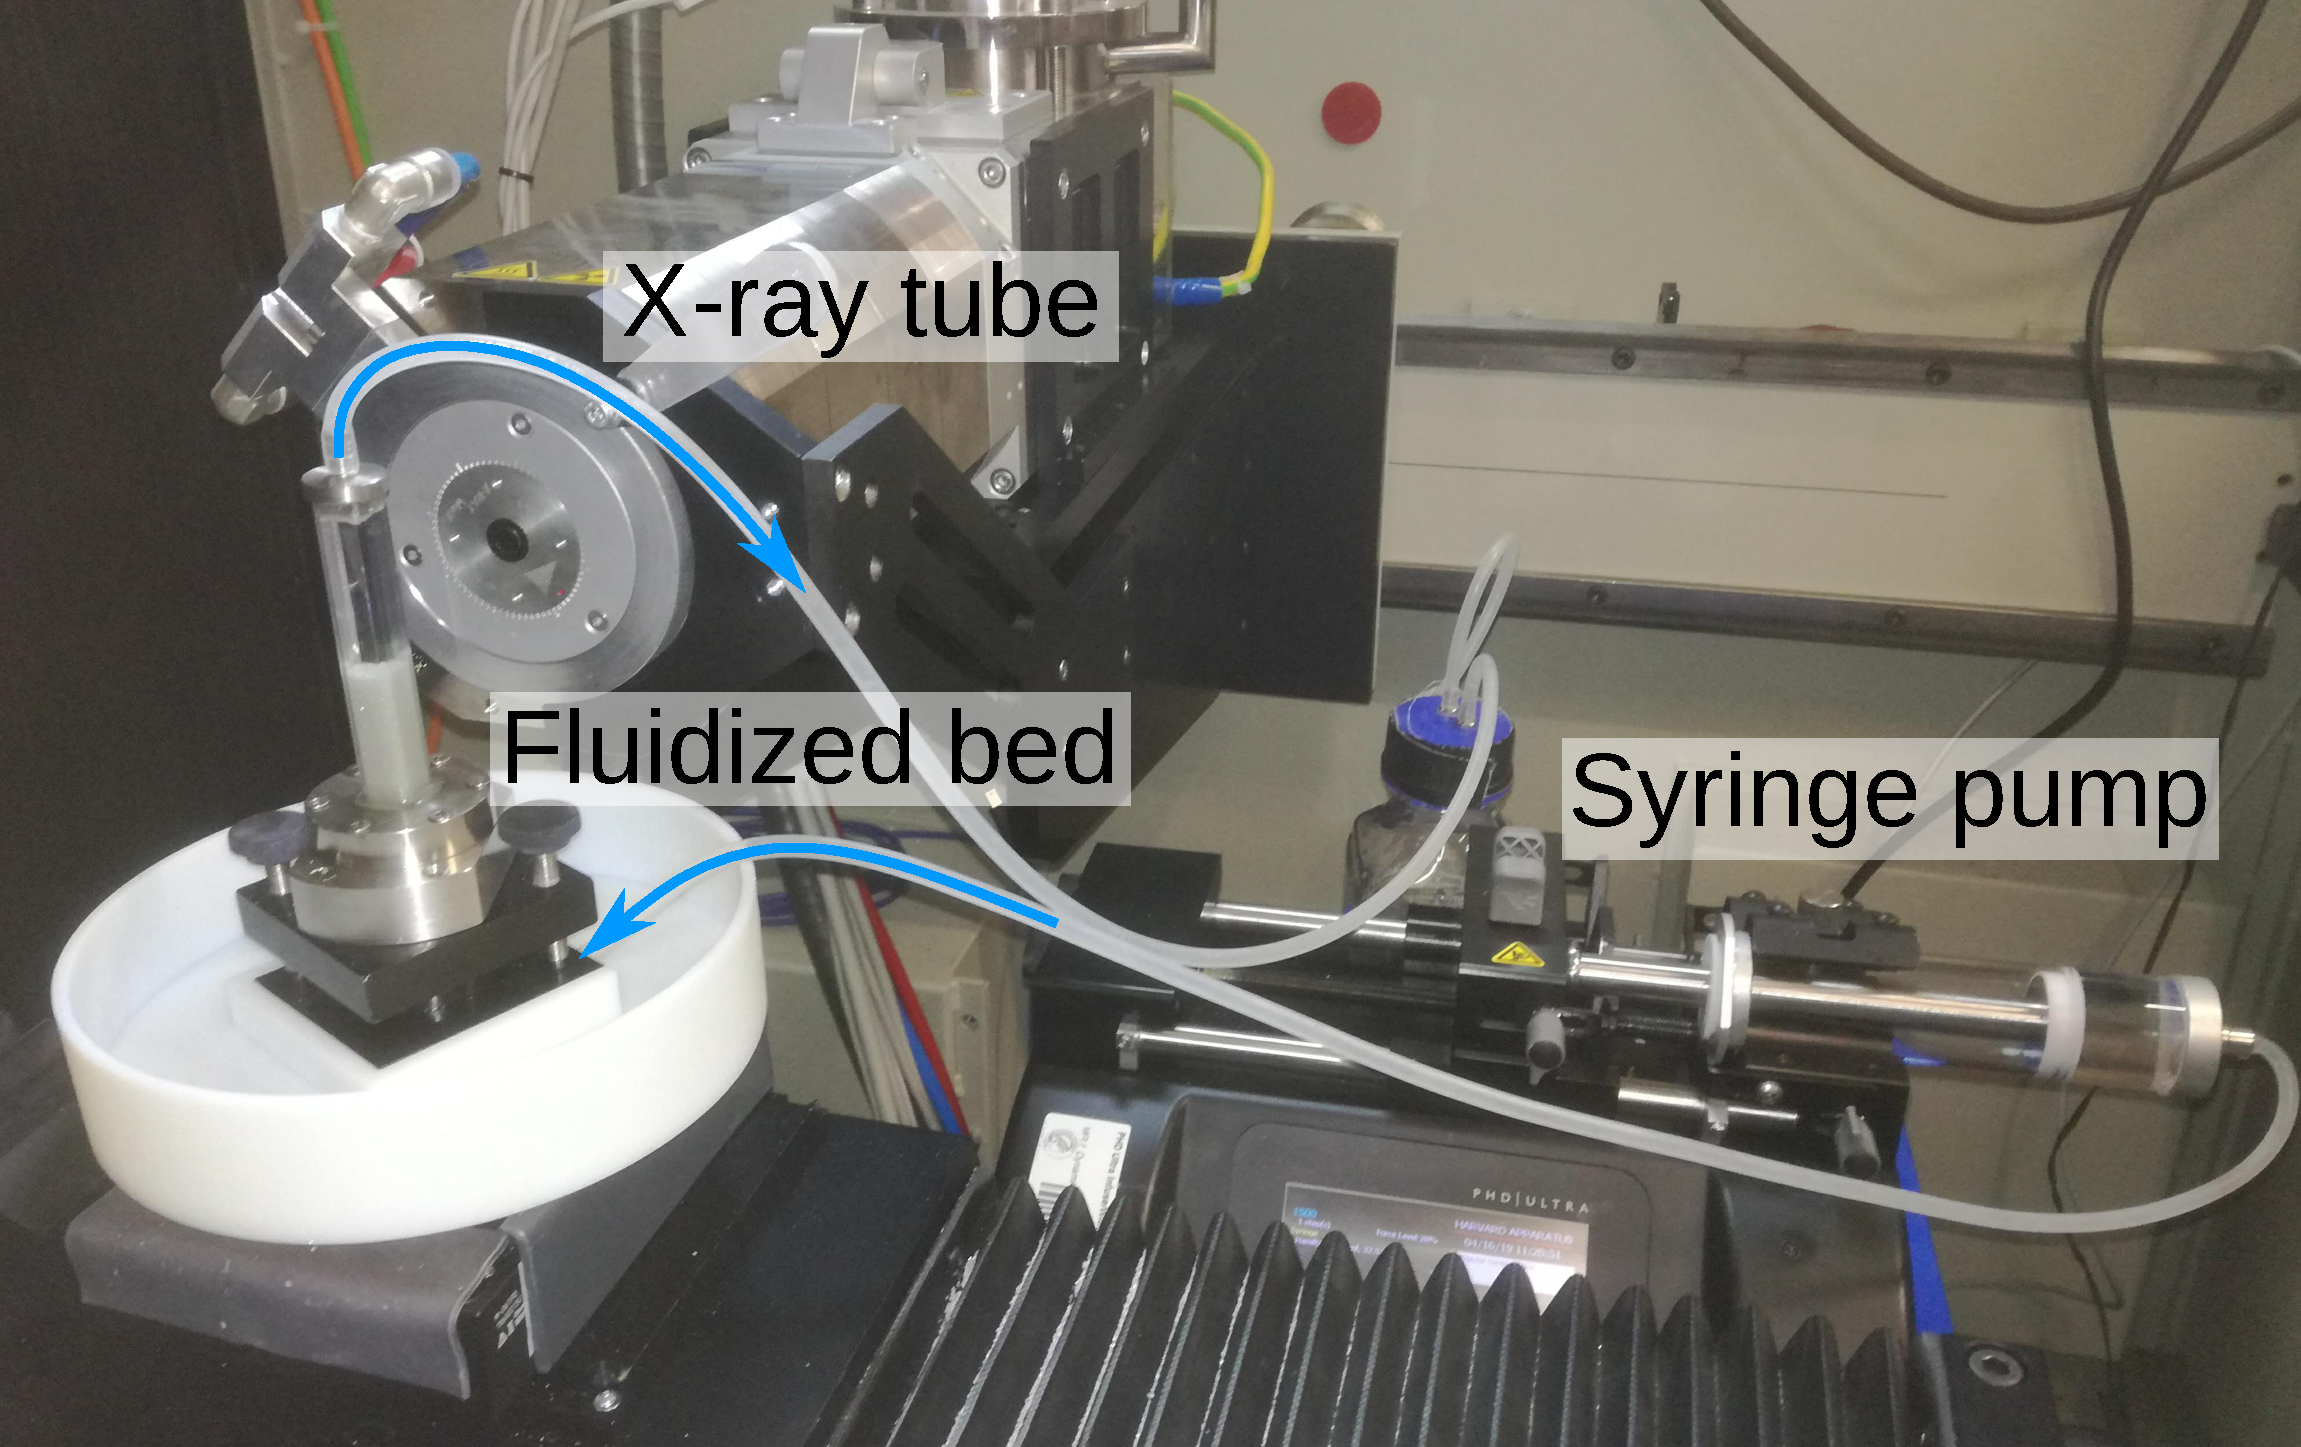
\includegraphics[width=\textwidth]{Sources/sedimenting_bed/Photo_fluidized_bed.pdf}
}
\only<2>{
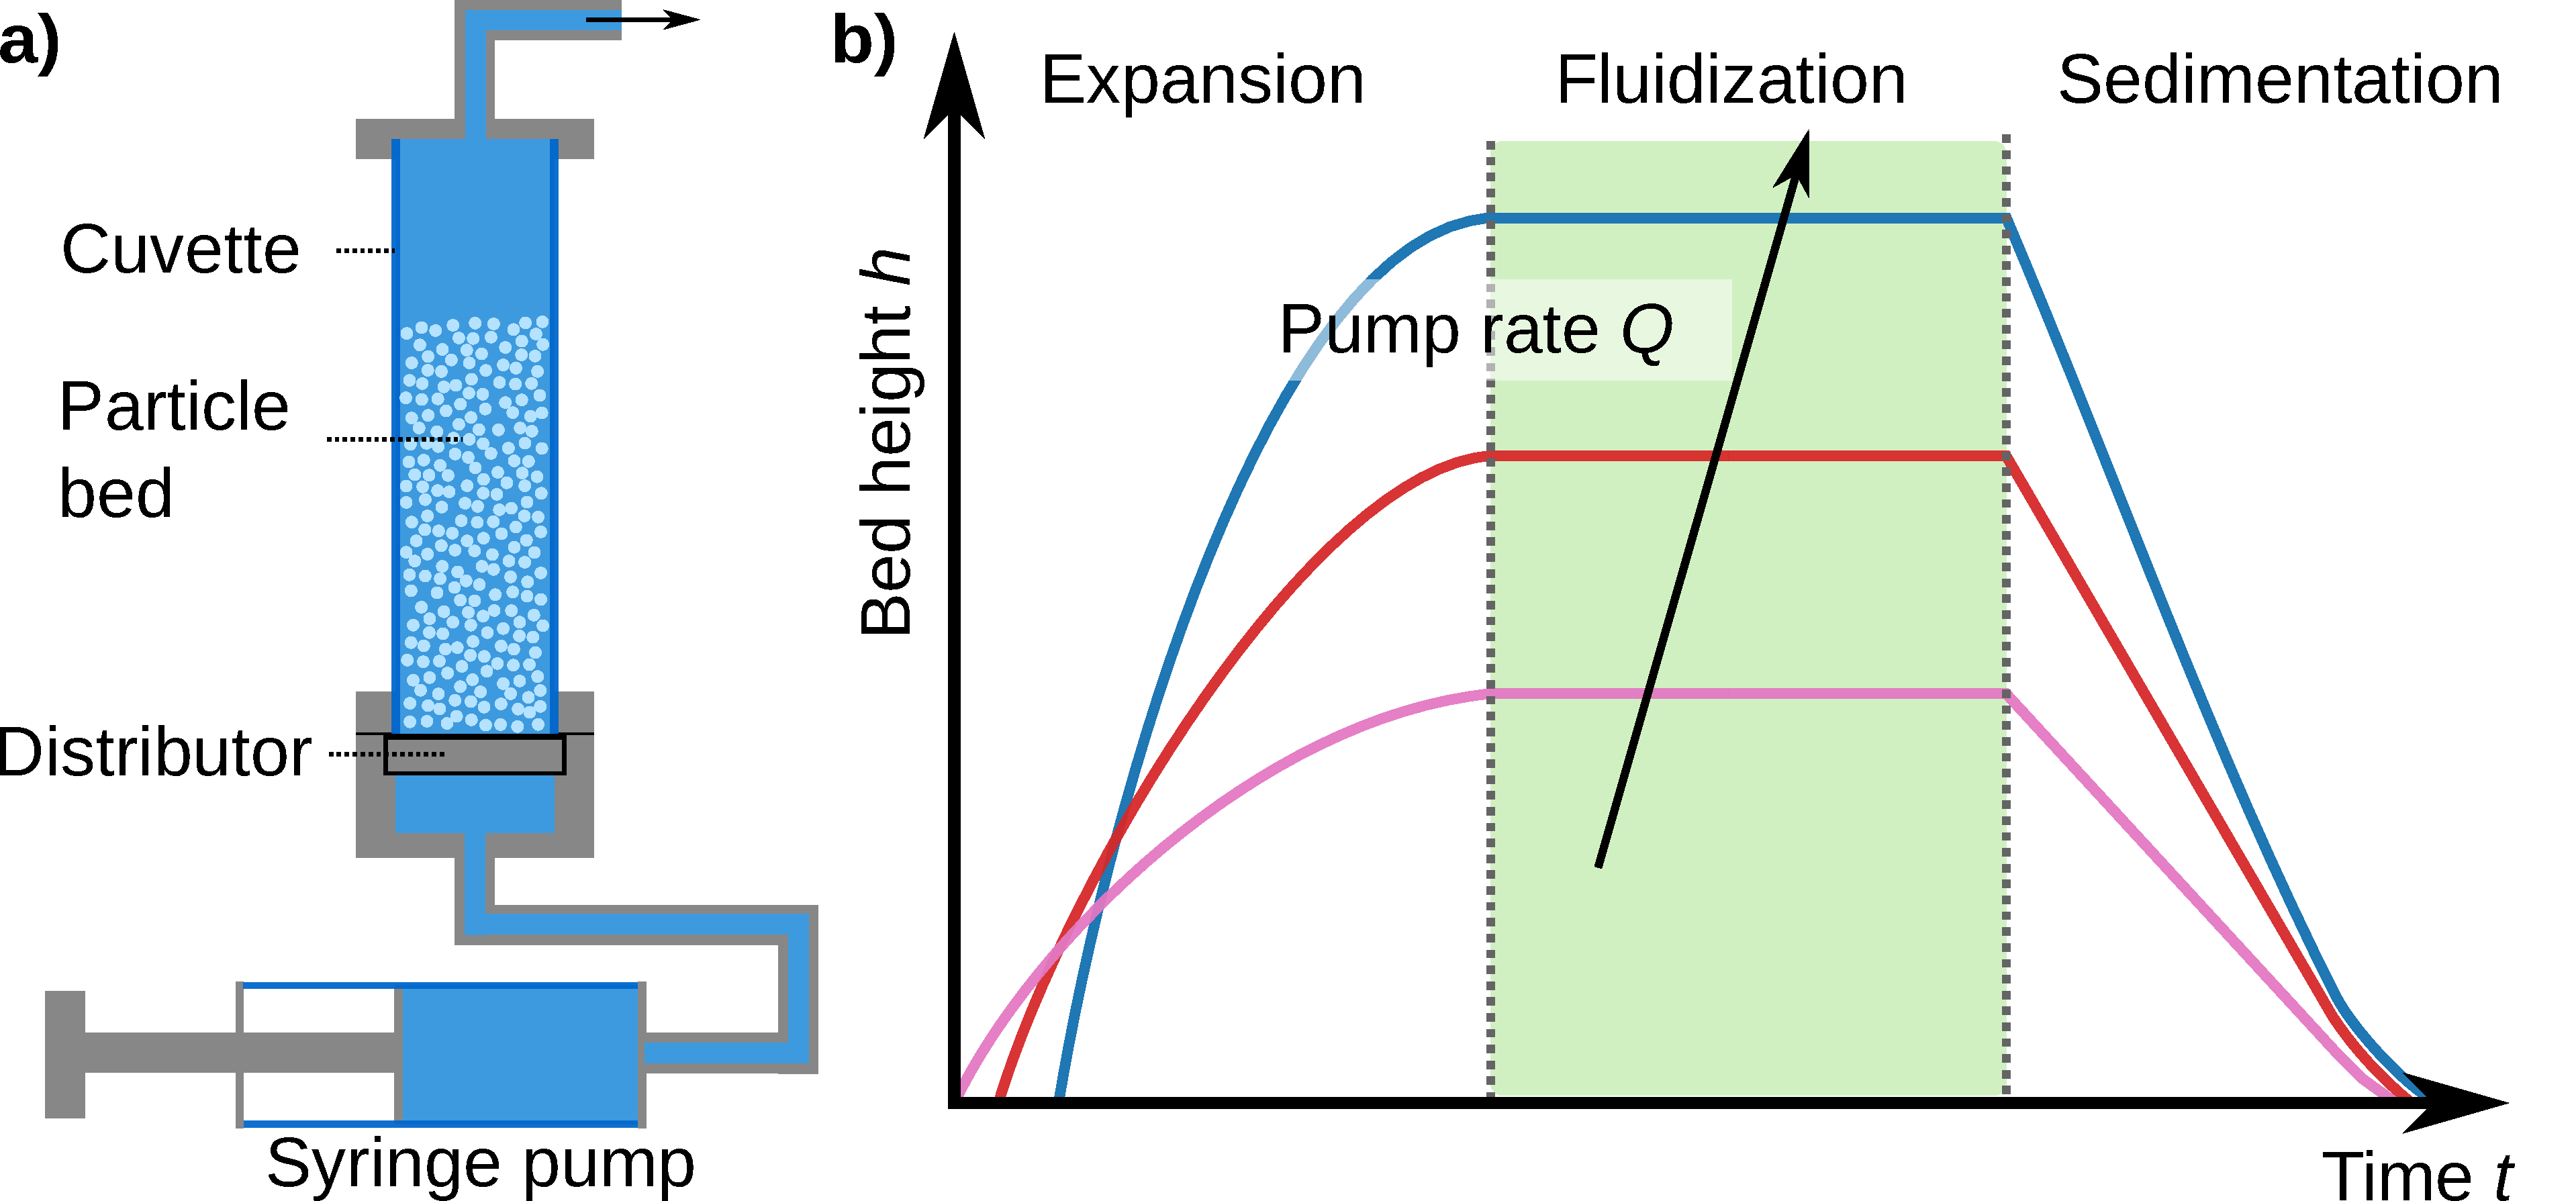
\includegraphics[width=\textwidth]{Sources/sedimenting_bed/setup-fluidized_bed_fluidized.pdf}}
\end{textblock}	

\begin{textblock}{0.35}(0.62,0.5)	
\only<2>{
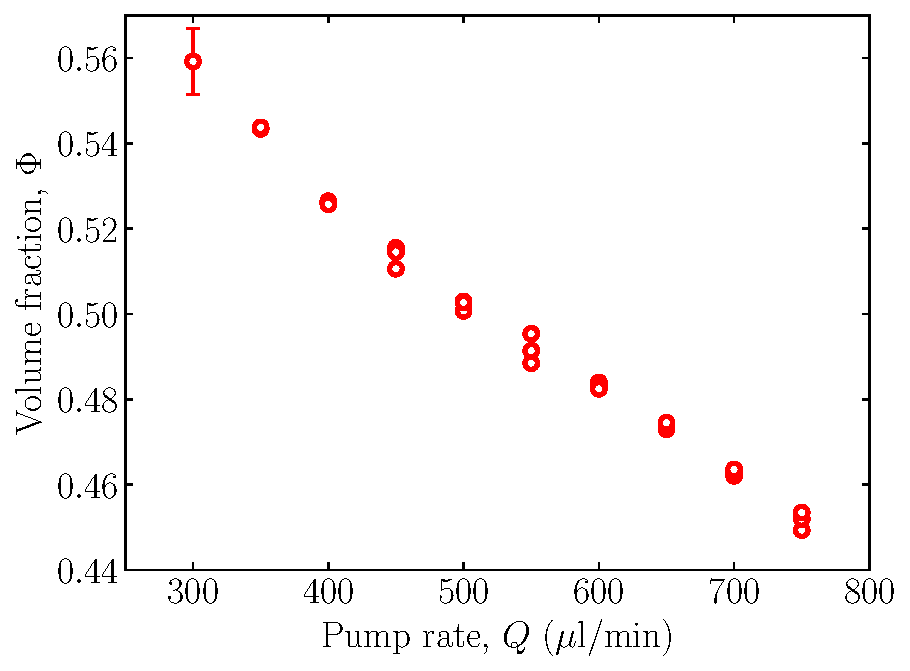
\includegraphics[width=\textwidth]{Sources/sedimenting_bed/Phi_vs_pump_rate.pdf}}
\end{textblock}


\begin{textblock}{0.3}(0.66,0.1)	
\visible<2->{
	
	\fbox{\parbox{\textwidth}{
			\centering
			video of bed}}}
\end{textblock}
}



\frame{
	\begin{tikzpicture}[remember picture,overlay]
	\fill[blue1]
	(current page.north west) rectangle ([xshift=0.51\textwidth,yshift=0.28\textheight]current page.west|-{pic cs:end});
	\end{tikzpicture}
	
	\begin{textblock}{0.5}(0.02,0.03)
		\textcolor{white}{
			\Large Experimental validation of X-DFA: Sedimenting particle suspension}
	\end{textblock}
	
	
	
	
	\begin{textblock}{0.6}(0.02,0.2)
		\centering
		\visible<1->{
			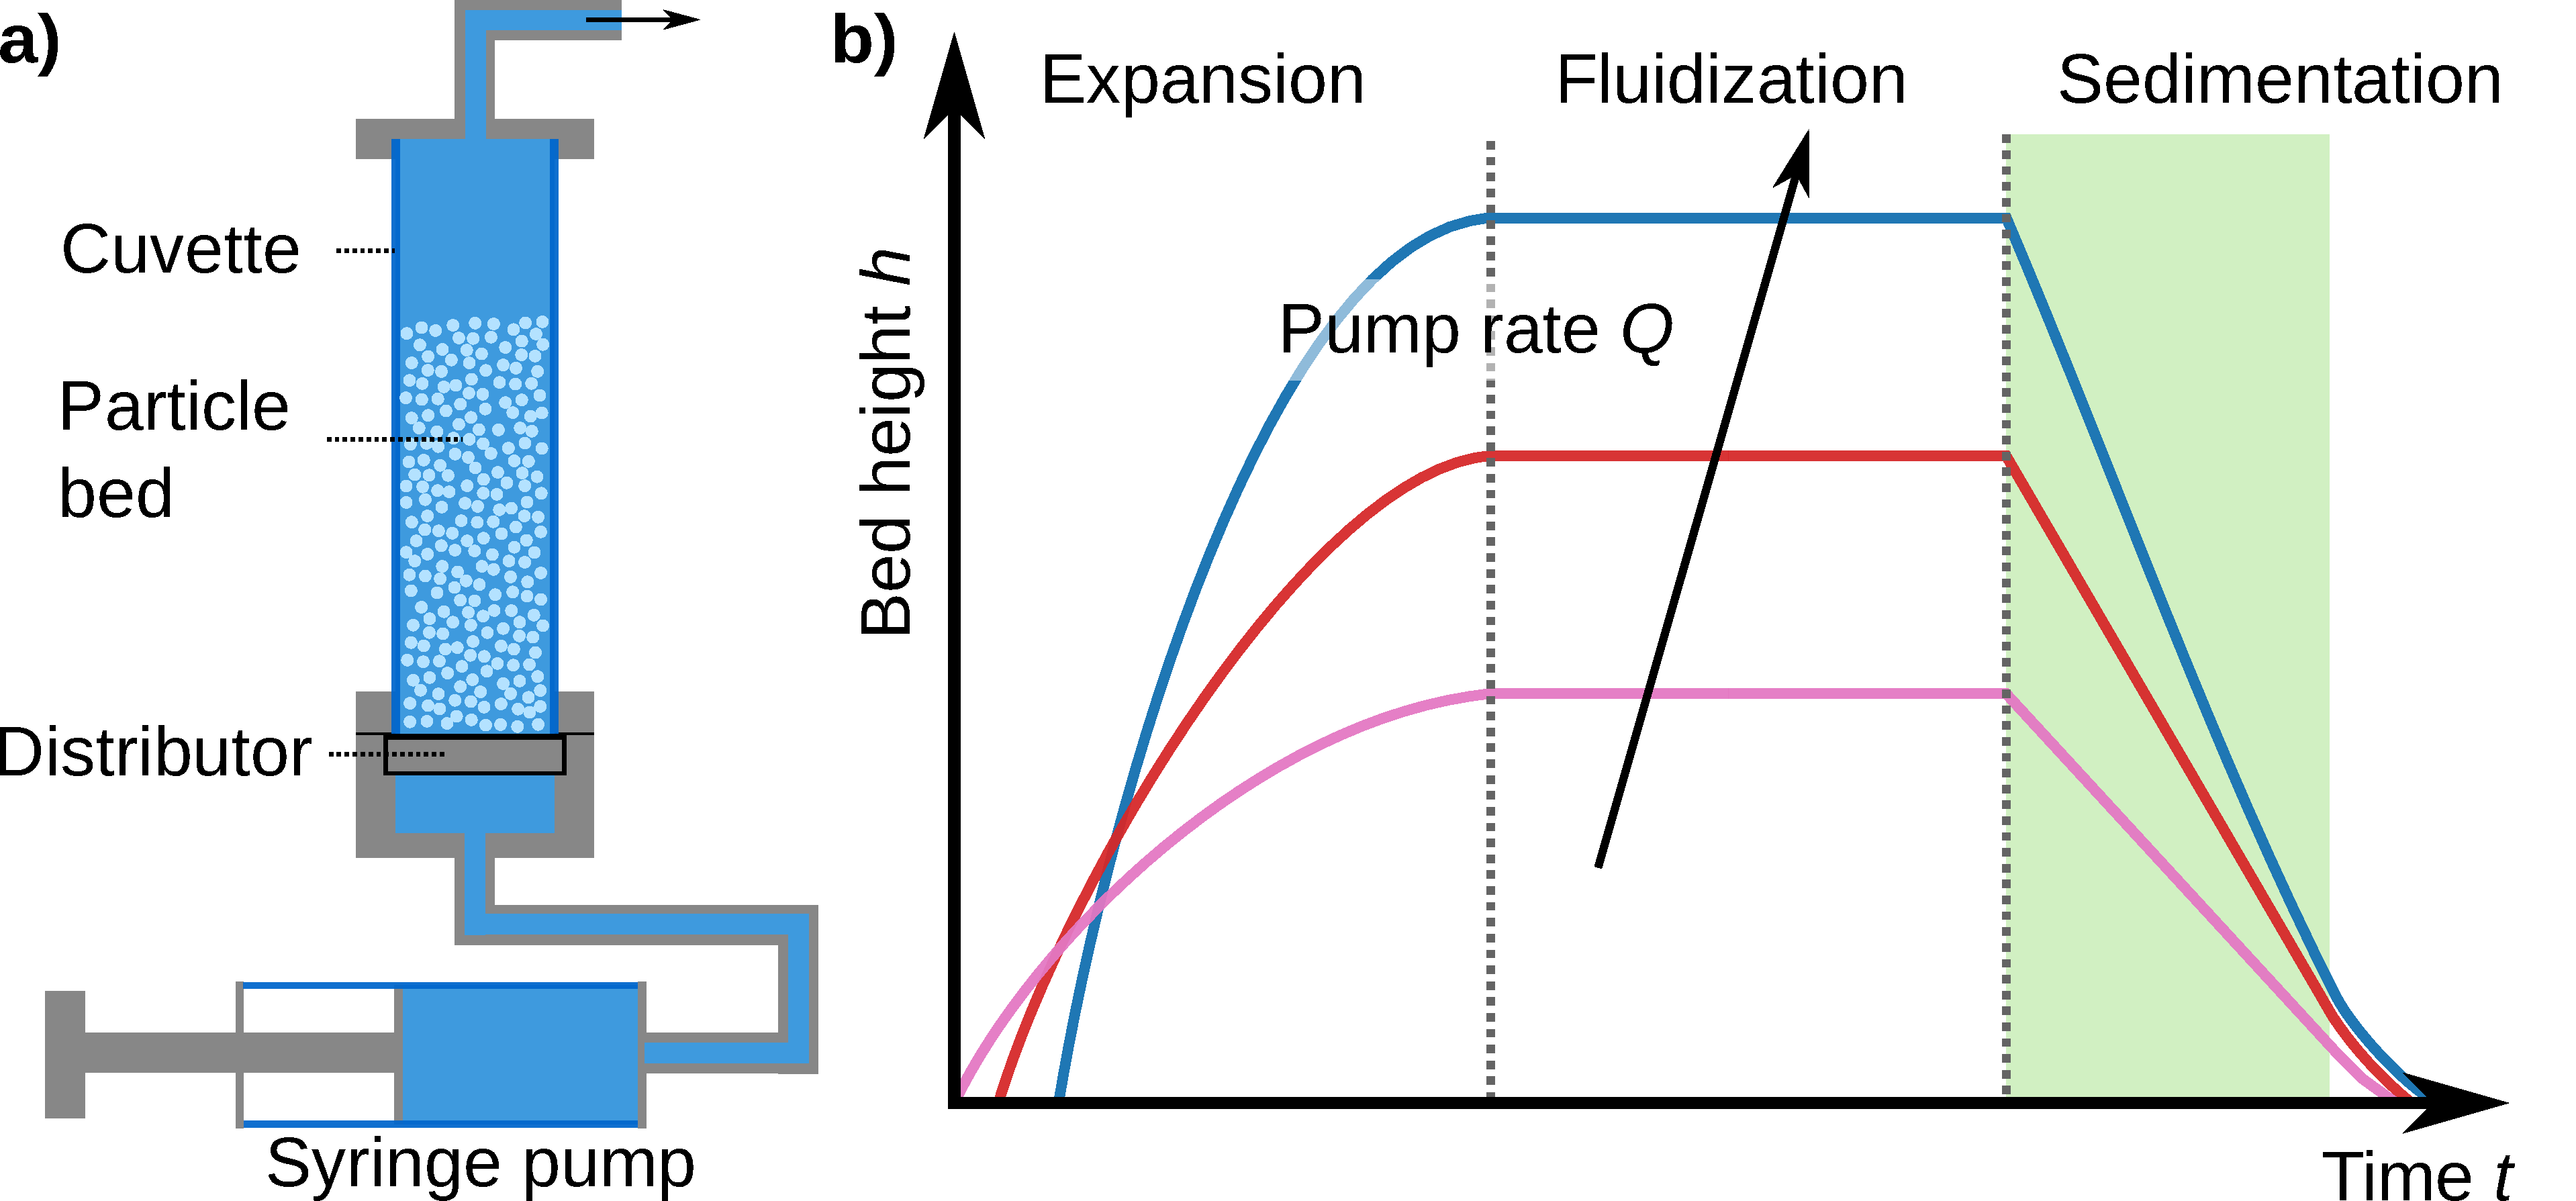
\includegraphics[width=\textwidth]{Sources/sedimenting_bed/setup-fluidized_bed.pdf}}
	\end{textblock}	
	
	\begin{textblock}{0.35}(0.62,0.5)	
		\only<2>{
			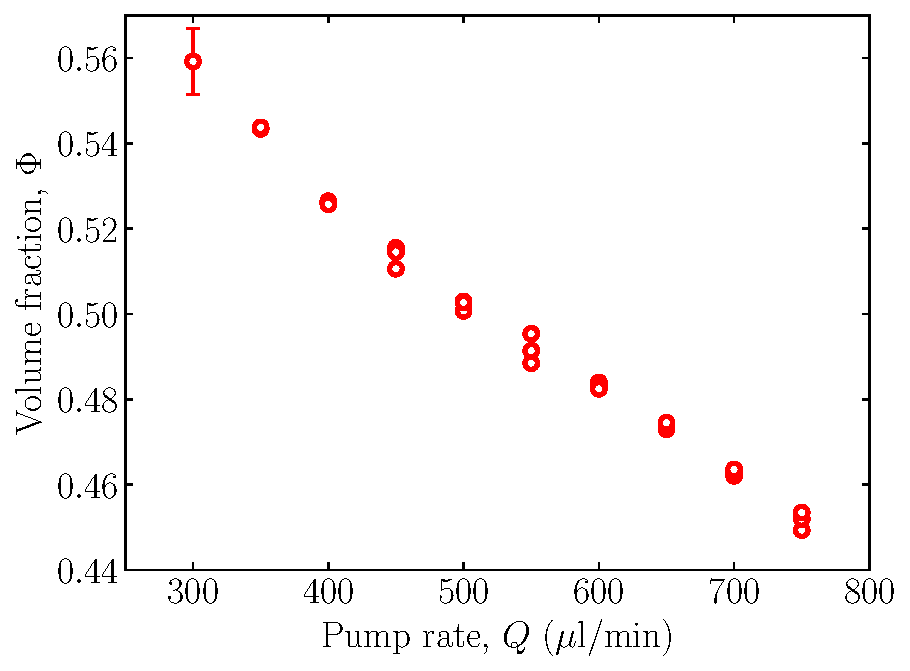
\includegraphics[width=\textwidth]{Sources/sedimenting_bed/Phi_vs_pump_rate.pdf}}
	\end{textblock}
	
	
	\begin{textblock}{0.3}(0.66,0.2)	
		\visible<2->{
			
			\fbox{\parbox{\textwidth}{
					\centering
					video of bed}}}
	\end{textblock}
	
	\begin{textblock}{0.3}(0.66,0.2)
		\fbox{\parbox{\textwidth}{
				\movie[width = \textwidth, poster]
				{}
				{Sources/sedimenting_bed/tracked_edge.avi}}}
	\end{textblock}
}


%%%%%%%%%%%%%%%%%%%%%%%%%%%%%%%%%%%%%%%%%%%%%%%%%%%%%%%%%%%%%%%%%%%%%%%%%%%%%%%%%%%%%%%%%%%%%%%%%%%%%%%%%%%
%\frame{
%\frametitle{Tracking of particle front}
%
%\begin{textblock}{0.9}(0.05,0.1)	
%\centering
%\only<1>{
%\includegraphics[width=0.8\textwidth]
%{Sources/sedimenting_bed/steepest_gradient_gv_profile.pdf}}
%\end{textblock}
%}
%
%\frame{
%\frametitle{Tracking of particle front}
%\begin{textblock}{0.7}(0.15,0.1)	
%	\centering
%	\only<1>{
%		\includegraphics[width=\textwidth]
%		{Sources/sedimenting_bed/setup-sketch-distortion.pdf}}
%\end{textblock}
%
%
%\begin{textblock}{0.9}(0.05,0.5)
%\only<1>{
%\vspace{-0.5cm}
%\centering
%\includegraphics[width=0.8\textwidth]
%{Sources/sedimenting_bed/image_transfer_function3_track_front_midplane.pdf}}
%\end{textblock}
%}
%
%\frame{
%\frametitle{Tracking of particle front}
%\begin{textblock}{0.9}(0.05,0.1)	
%	\centering
%	\only<1>{
%		\includegraphics[width=0.5\textwidth]
%		{Sources/sedimenting_bed/steepest_gradient_gv_profile.pdf}}
%\end{textblock}
%
%\begin{textblock}{0.35}(0.02,0.5)	
%\centering
%\visible<1->{
%\includegraphics[width=\textwidth]
%{Sources/sedimenting_bed/plot_extract_edge_pos_mid_plane.png}}
%\end{textblock}
%
%
%\begin{textblock}{0.35}(0.52,0.5)	
%\centering
%\visible<1->{
%\includegraphics[width=\textwidth]
%{Sources/sedimenting_bed/lin_fit_y-pos_vs_time.png}}
%\end{textblock}
%}
%
%
%
%
%
%%%%%%%%%%%%%%%%%%%%%%%%%%%%%%%%%%%%%%%%%%%%%%%%%%%%%%%%%%%%%%%%%%%%%%%%%%%%%%%%%%%%%%%%%%%%%%%%%%%%%
%\frame{
%	\frametitle{X-DFA for sedimenting particles}
%	\begin{textblock}{0.9}(0.05,0.1)	
%		\centering
%		\includegraphics[width=0.9\textwidth]
%		{Sources/sedimenting_bed/image_structure_func.pdf}
%	\end{textblock}	
%
%	\begin{textblock}{0.2}(0.51,0.25)
%		\visible<2->{
%		\colorbox{blue1}{\textcolor{white}{$I(x,t)$}}
%		}
%	\end{textblock}
%
%	\begin{textblock}{0.2}(0.75,0.15)
%	\visible<3->{
%		\colorbox{blue1}{\textcolor{white}{$|\Delta I(x,t)|^2$}}
%		}
%	\end{textblock}
%
%	\begin{textblock}{0.2}(0.71,0.7)
%	\visible<4->{
%		\colorbox{blue1}{\textcolor{white}{$\langle |\Delta \mathscr{F} (\Delta I)|^2 \rangle_t$}}
%		}
%	\end{textblock}
%}
%
%\frame{
%\frametitle{X-DFA for sedimenting particles}
%
%\begin{textblock}{0.9}(0.05,0.05)
%	\begin{align}
%	f(q,\tau) = 
%	\cos(q \langle v_\text{s} \rangle \tau)
%	\exp\left(- \frac{1}{2} q^2 \delta v^2 \tau^2 \right)
%	\nonumber
%	\end{align}
%	\centering
%	$\langle v_\text{s} \rangle = \langle \Delta r \rangle / \tau_\nu, 
%	\langle \delta v \rangle = \langle \delta r \rangle / \tau_{\delta \nu}$
%\end{textblock}
%
%\begin{textblock}{0.45}(0.025,0.4)	
%	\centering
%	\includegraphics[width=\textwidth]
%	{Sources/sedimenting_bed/fqt_tq.pdf}
%\end{textblock}
%
%\begin{textblock}{0.45}(0.5,0.4)	
%	\centering
%	\includegraphics[width=\textwidth]
%	{Sources/sedimenting_bed/tau_vs_q.pdf}
%\end{textblock}
%}
%
%\frame{	
%\frametitle{Richardson-Zaki law}
%
%\begin{textblock}{0.45}(0.025,0.1)	
%	\centering
%	\includegraphics[width=\textwidth]
%	{Sources/sedimenting_bed/Phi_vs_pump_rate.pdf}
%\end{textblock}
%
%\begin{textblock}{0.45}(0.5,0.2)
%	\[ \frac{\langle v \rangle_\text{front}}{v_\text{Stokes}} = (1-\Phi)^n \]
%\end{textblock}
%
%\begin{textblock}{0.45}(0.5,0.35)	
%	\centering
%	\includegraphics[width=\textwidth]
%	{Sources/sedimenting_bed/Sed_vel_vs_Phi_fit_Richardson_Zaki.pdf}
%\end{textblock}
%}
%%%%%%%%%%%%%%%%%%%%%%%%%%%%%%%%%%%%%%%%%%%%%%%%%%%%%%%%%%%%%%%%%%%%%%%%%%%%%%%%%%%%%%%%%%%%%%%%%%%%
%\frame{
%	\frametitle{X-DFA: Requirement of linear space invariant imaging}
%	
%	\begin{textblock}{0.6}(0.0,0.08)	
%		\begin{align}
%		I(\mathbf{r},t) = I_0 + \int \mathsf{d}\mathbf{r}' \ \mathsf{d}z'
%		T(\mathbf{r}-\mathbf{r}',-z') c(\mathbf{r}',z',t)
%		\nonumber
%		\end{align}
%	\end{textblock}
%	
%
%	
%	\begin{textblock}{0.5}(0.5,0.45)
%		\centering
%		\includegraphics[width=0.8\textwidth]
%		{Sources/sedimenting_bed/I_over_I0_vs_Phi.pdf}
%	\end{textblock}
%
%	\begin{textblock}{0.9}(0.05,0.15)	
%	\centering
%	\includegraphics[width=0.7\textwidth]
%	{Sources/sedimenting_bed/image_transfer_function1.pdf}
%	\end{textblock}
%	
%
%}
%
%
%
%
%%%%%%%%%%%%%%%%%%%%%%%%%%%%%%%%%%%%%%%%%%%%%%%%%%%%%%%%%%%%%%%%%%%%%%%%%%%%%%%%%%%%%%%%%%%%%%%%%%%%%%%%%%%
%\frame{
%\frametitle{Front tracking vs.\ X-DFA}
%\begin{textblock}{0.45}(0.02,0.1)	
%\centering
%\visible<1->{
%\includegraphics[width=\textwidth]
%{Sources/sedimenting_bed/Sedimentation_velocites_v_front_vs_v_X-DFA.pdf}
%}
%\vspace{-0.3cm}
%$\langle v\rangle_\text{xdfa} > \langle v \rangle_\text{front}$ by 9.4\%
%\end{textblock}
%
%\begin{textblock}{0.5}(0.5,0.15)
%	\centering
%	\includegraphics[width=0.8\textwidth]
%	{Sources/sedimenting_bed/creeping_boundary_flow.pdf}
%\end{textblock}
%
%\begin{textblock}{0.5}(0.5,0.75)
%	\centering
%	\href{run:Sources/sedimenting_ved/sample_selection_10_600ul_per_min_Matthias.avi}
%	{\textcolor{red}{sample video}}
%\end{textblock}
%}
%
%\frame{
%\frametitle{Estimate width of boundary layer}
%\begin{textblock}{0.45}(0.02,0.1)	
%	\centering
%	\visible<1->{
%		\includegraphics[width=\textwidth]
%		{Sources/sedimenting_bed/creeping_boundary_flow.pdf}
%	}
%	$\langle v\rangle_\text{xdfa} > \langle v \rangle_\text{front}$ by 9.4\%
%\end{textblock}
%
%\begin{textblock}{0.5}(0.5,0.1)
%	$\langle v\rangle_\text{xdfa}$ takes \textcolor{red}{two} layers into account\\
%	$\langle v \rangle_\text{front}$ takes \textcolor{royalblue}{four} layers into account\\[0.3cm]
%	
%	\includegraphics[width=0.9\textwidth]
%	{Sources/sedimenting_bed/sketch_boundary_flow.pdf}\\[0.3cm]
%%	\vspace{0.6cm}
%	\textbf{Estimation:}\\
%	Boundary velocity = 0\\
%	Else = const.\\
%	$\rightarrow b \approx 3$ particle diameters
%\end{textblock}
%
%}
%
%\frame{
%\begin{textblock}{1.}(0.0,0.0)
%	\includegraphics[width=\textwidth]
%	{Sources/sedimenting_bed/whiteboard.jpg}
%\end{textblock}
%
%\begin{textblock}{0.8}(0.2,0.3)
%	\colorbox{blue1}{\Huge \textcolor{white}{Thank you for your attention!}}
%\end{textblock}
%}



